\documentclass{article}
 
\usepackage{amsmath}
\usepackage{amssymb}
\usepackage{listings}
\usepackage{graphicx}
\usepackage{subcaption}
\usepackage{mwe}
\usepackage{float}
\usepackage{epstopdf}
\usepackage[top=1.5in, bottom=1in, left=1in, right=1in]{geometry}


\title{Project 2 Advanced Land Finding Writeup}

\begin{document}
\maketitle
\section{Project Goals}

The goals / steps of this project are the following:\\\\
* Compute the camera calibration matrix and distortion coefficients given a set of chessboard images.\\
* Apply a distortion correction to raw images.\\
* Use color transforms, gradients, etc., to create a thresholded binary image.\\
* Apply a perspective transform to rectify binary image ("birds-eye view").\\
* Detect lane pixels and fit to find the lane boundary.\\
* Determine the curvature of the lane and vehicle position with respect to center.\\
* Warp the detected lane boundaries back onto the original image.\\
* Output visual display of the lane boundaries and numerical estimation of lane curvature and vehicle position.\\

\section{Write up}
In this section I will go over the pipeline code in project2.py
\subsection{Camera Calibration and Distortion Correction} 
The first step is to calibrate the camera using the provided figures using the defined function $cameraCalibration$ and $undistort$. \\
The first function defines object and find image points for camera calibration using $cv2.findChessboardCorners()$. The second function creates undistort images witg $cv2.calibrateCamera()$ and $cv2.undistort()$. An example of the figure before and after distortion correction is shown in Figure \ref{fig1a} , Figure \ref{fig1b}, Figure \ref{fig2a} and Figure \ref{fig2b}.

\begin{figure}
     \centering
     \begin{subfigure}[b]{0.4\textwidth}
         \centering
         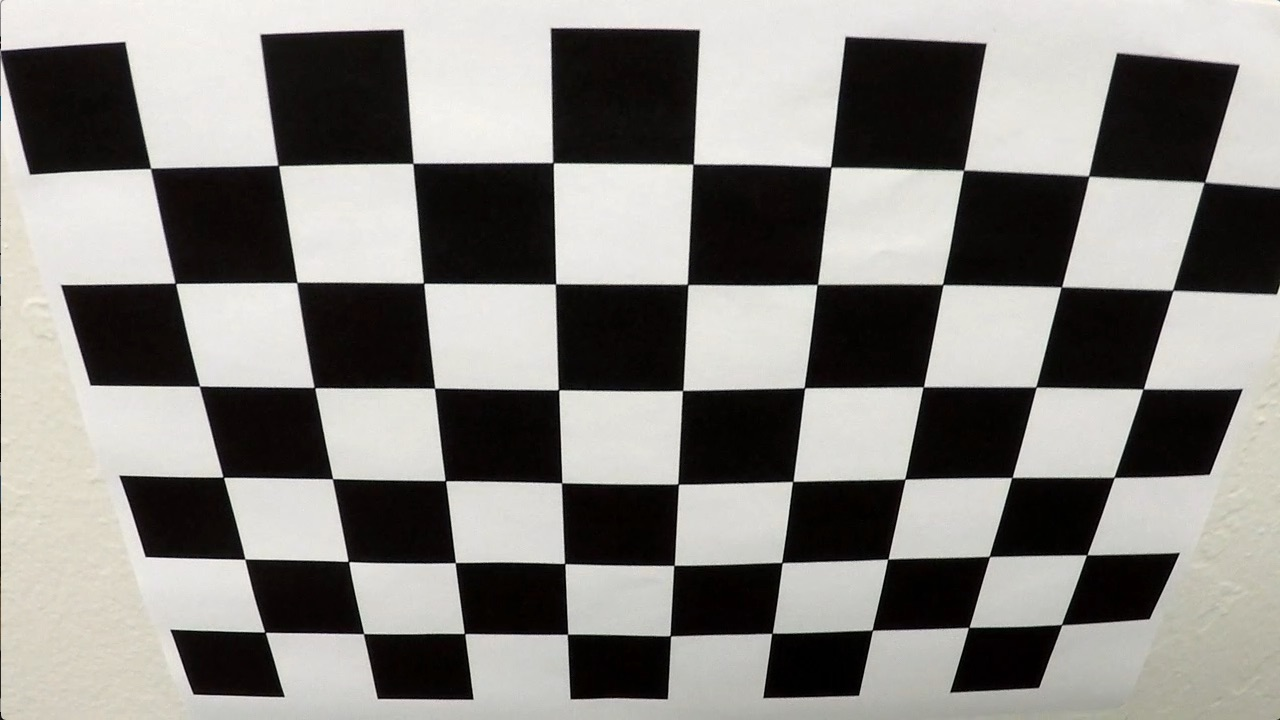
\includegraphics[width=\textwidth]{../camera_cal/calibration2.jpg}
         \caption{Before Distortion Correction}
         \label{fig1a}
     \end{subfigure}
     \hfill
     \begin{subfigure}[b]{0.4\textwidth}
         \centering
         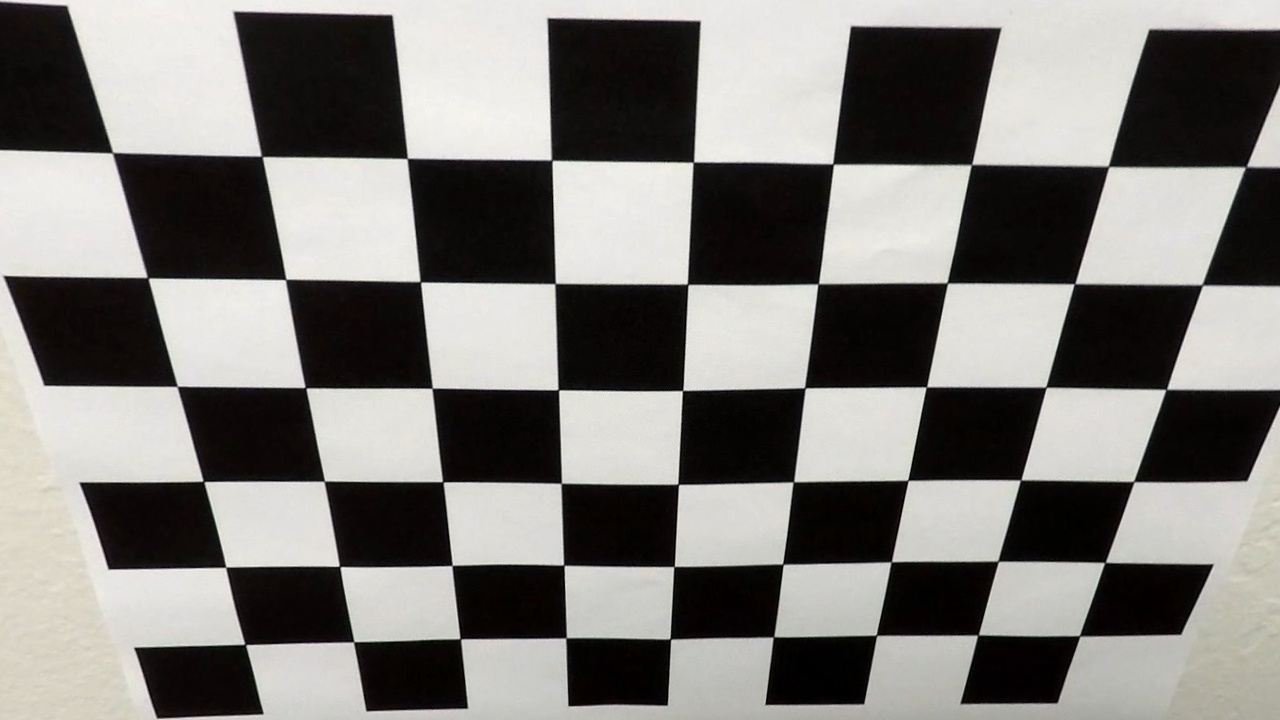
\includegraphics[width=\textwidth]{../output_images/undistort/alibration2.jpg}
         \caption{After Distortion Correction}
         \label{fig1b}
     \end{subfigure}
\end{figure}
\subsection{Create Color Thresholded Image} 

\begin{figure}
     \centering
     \begin{subfigure}[b]{0.4\textwidth}
         \centering
         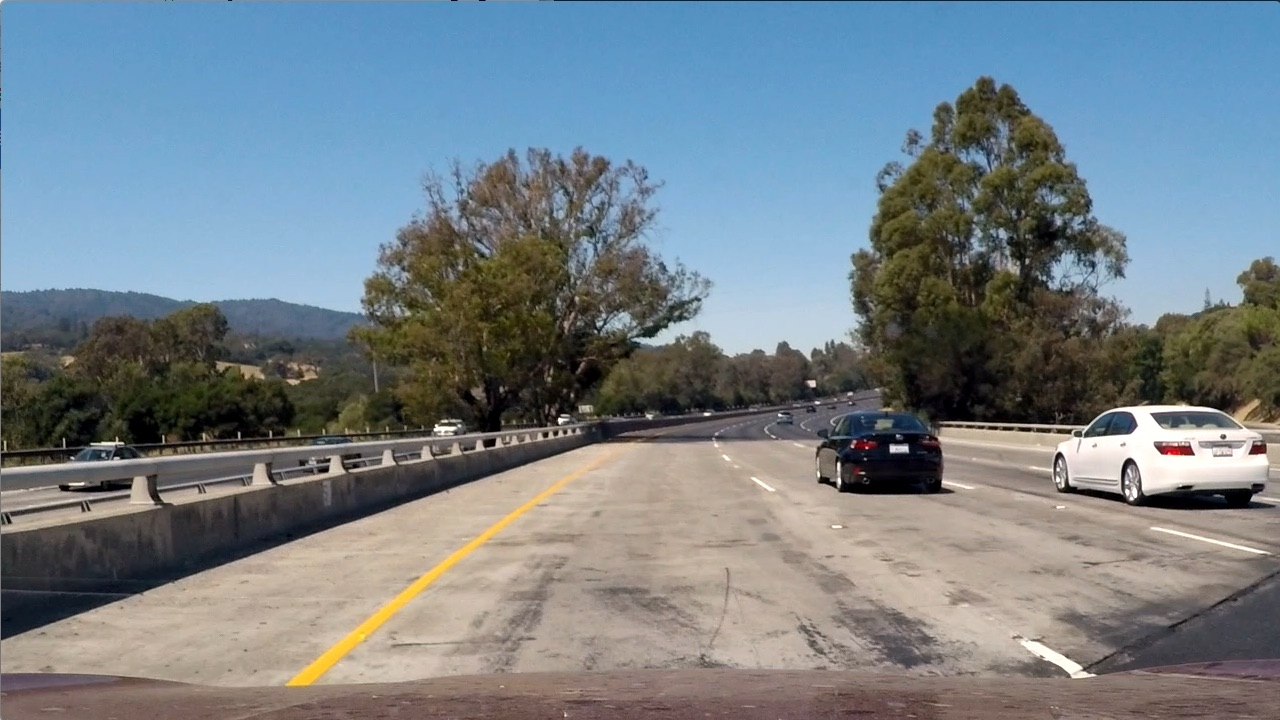
\includegraphics[width=\textwidth]{../test_images/test1.jpg}
         \caption{Before Distortion Correction}
         \label{fig2a}
     \end{subfigure}
     \hfill
     \begin{subfigure}[b]{0.4\textwidth}
         \centering
         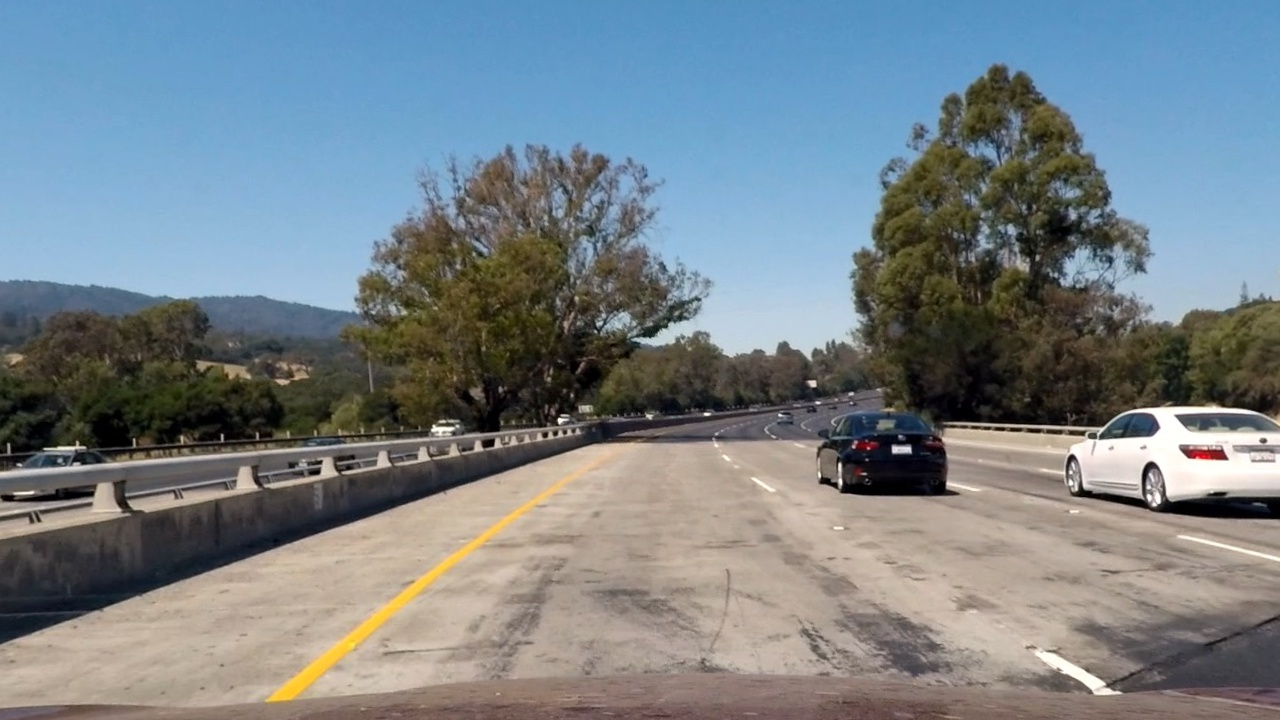
\includegraphics[width=\textwidth]{../output_images/undistort/test1.jpg}
         \caption{After Distortion Correction}
         \label{fig2b}
     \end{subfigure}
\end{figure}
The function $thresholdImage$ is used to create the binary threshold images. It use threshold in HLS S-Channel and Sobel X direction to create the thresholded binary image for line detection.  Additionally a HLS L-Channel threshold is added to remove the dark tree shadow that also cross S-Channel threshold.\\\\
The final threshold values are $170<HLS_S<255$, $HLS_L>=100$ and $40<Sobel_x<100$, an example of the output is shown in Figure \ref{fig3}.\\

\begin{figure}[h!t]
\begin{center}
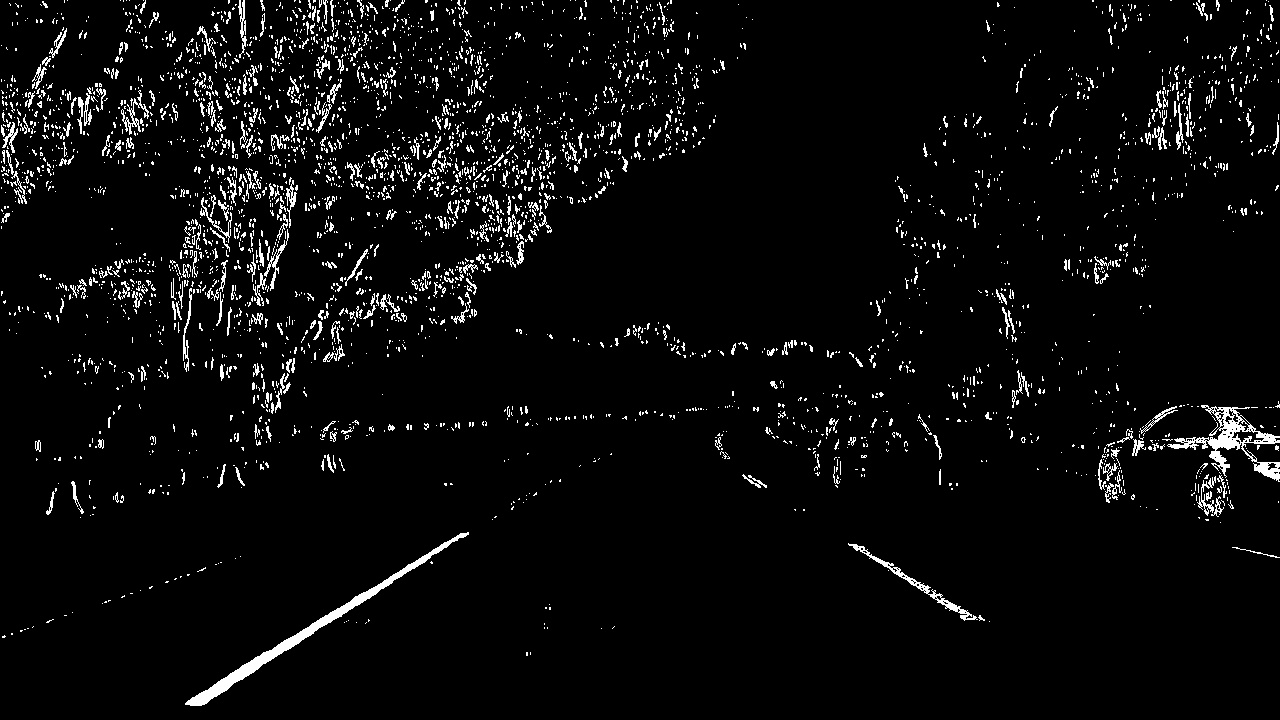
\includegraphics[width=0.75\textwidth]{../output_images/threshold/v2test5.jpg}
\caption{Binary Thresholded Output of Test Image 5}
\label{fig3}
\end{center}
\end{figure}

\subsection{Perspective Transform "Bird-Eye View"} 
The function $birdsEye$ is used to warp the image to bird-eye view. The key parameters source and destination points are defined in the following Table \ref{table1}. The values are verified by checking on a straight line as shown in Figure \ref{fig4}.\\

\begin{table}[h!t]
  \begin{center}
    \caption{Perspective Transform Parameters}
    \label{table1}
    \begin{tabular}{l|l} % <-- Alignments: 1st column left, 2nd middle and 3rd right, with vertical lines in between
      \textbf{Source Point} & \textbf{Destination Point}\\
      \hline
      (592,450) & (240,0)\\
      (688,450) & (1040,0)\\
      (1120,720) & (1040,720)\\
      (200,720) & (240,720)\\
    \end{tabular}
  \end{center}
\end{table}

\begin{figure}[h!t]
\begin{center}
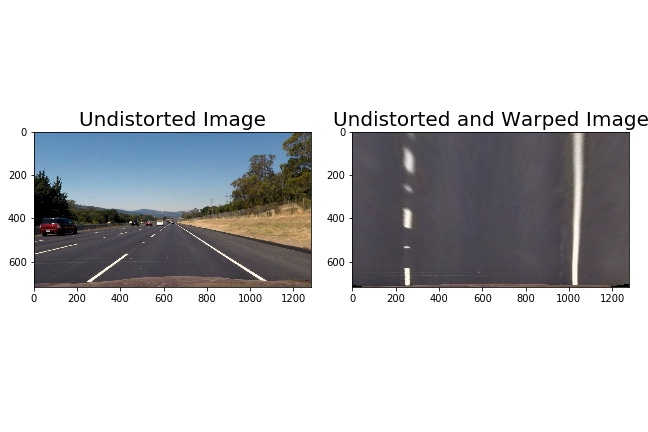
\includegraphics[width=0.75\textwidth]{../output_images/birdeye/straight_lines2.jpg}
\caption{Perspective Transform on Straight Road}
\label{fig4}
\end{center}
\end{figure}

\subsection{Polynomial Fit} 
The function $search_around_poly$ is the main one to warp the image to bird-eye view. Before that, the function $fit_firstPoly$ uses sliding window method (as shown in Figure \ref{fig5}) to find the line to calculate the first polynomial and update the variable $self.left\_fit$ and $self.right\_fit$.  After that, the line in the new frame is searched through with a smaller margin in an area based on the previous polynomial as  Figure \ref{fig6} shows. Then the calculated polynomial is shown in Figure \ref{fig7}.

\begin{figure}[h!t]
\begin{center}
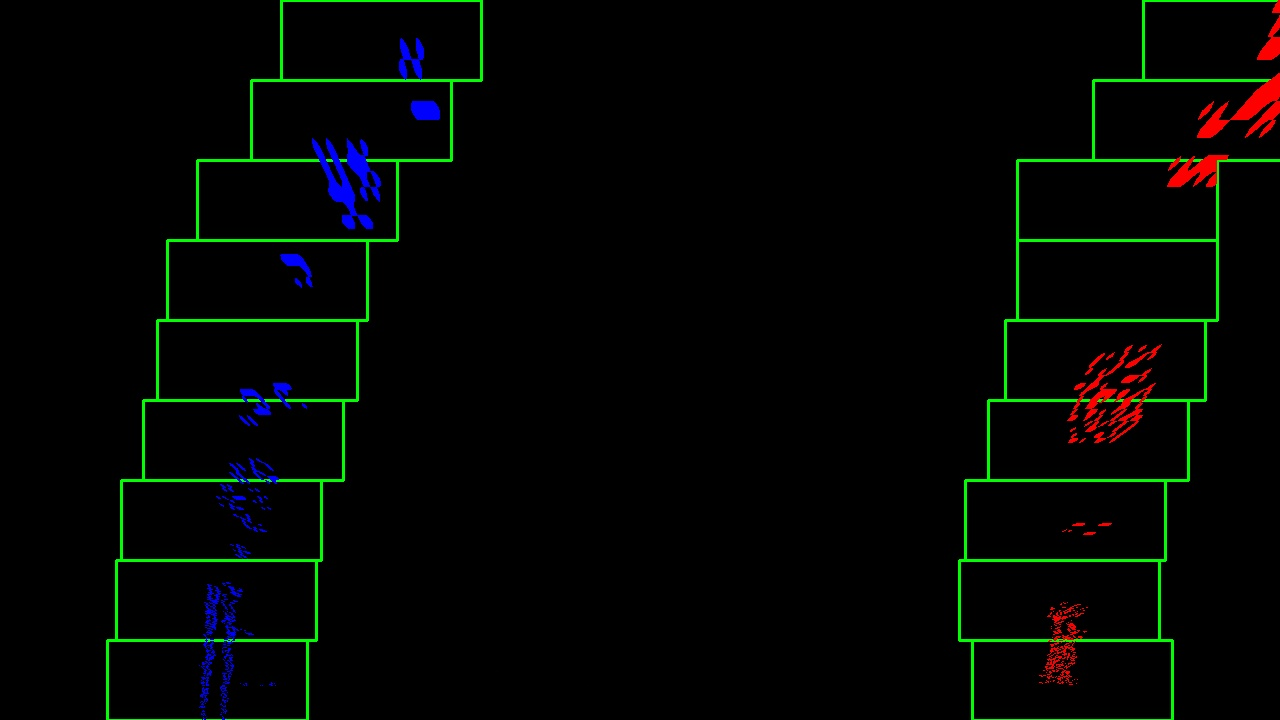
\includegraphics[width=0.75\textwidth]{../output_images/polynomialfit/test5.jpg}
\caption{Sliding Windows}
\label{fig5}
\end{center}
\end{figure}

\begin{figure}[h!t]
\begin{center}
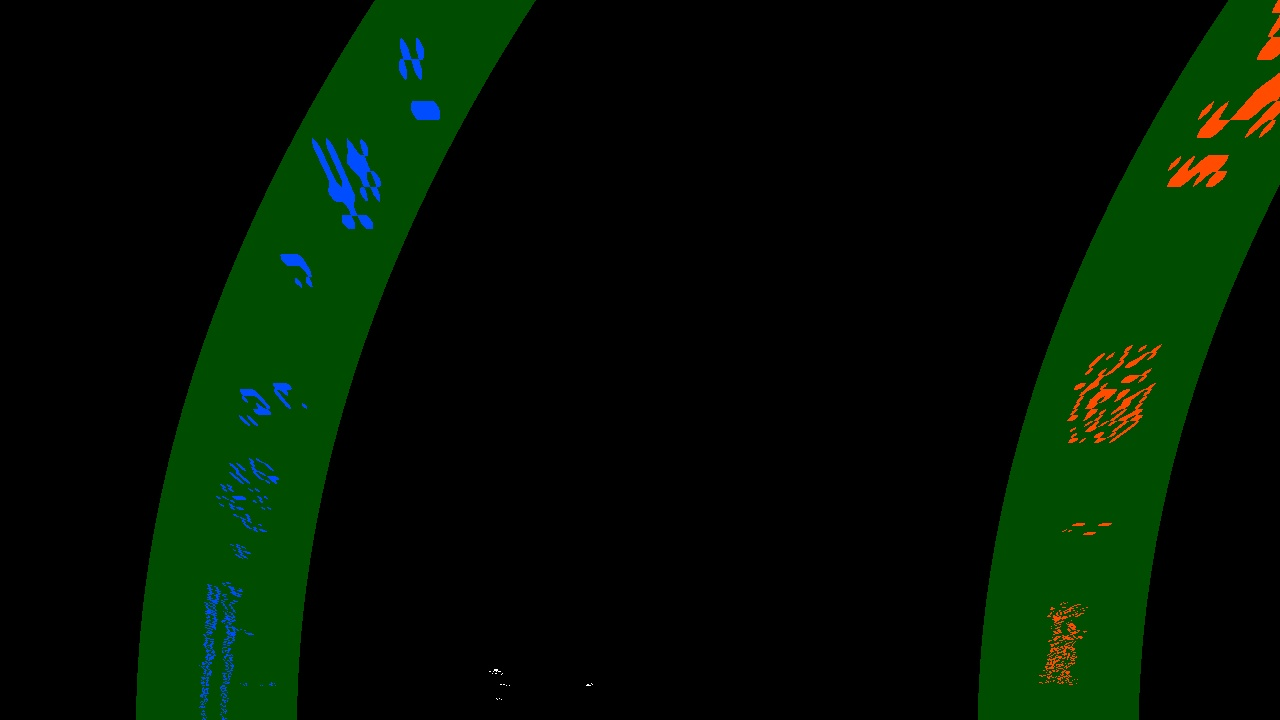
\includegraphics[width=0.75\textwidth]{../output_images/polynomialfit/v2test5.jpg}
\caption{Polynomial Area}
\label{fig6}
\end{center}
\end{figure}

\begin{figure}[h!t]
\begin{center}
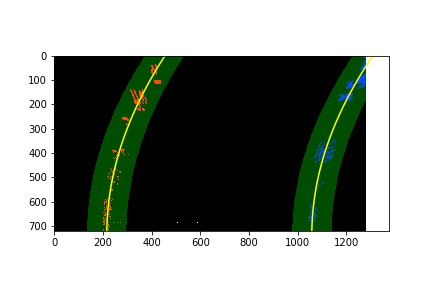
\includegraphics[width=0.75\textwidth]{../output_images/polynomialfit/v3test5.jpg}
\caption{Polynomial Visualization}
\label{fig7}
\end{center}
\end{figure}

\subsection{Curvature and Vehicle Position Calculation} 
Curvature is calculated in the function $measure\_curvature\_real$ through the following formula, where $A$ and $B$ are the coefficients in the polynomial and $y$ is the location at the bottom of the image.\\
\begin{equation}
R_{curve}=\frac{(1+(2Ay+B)^2)^{3/2}}{|2A|}
\end{equation}
Then the vehicle position is calculate in function $measure\_vehicle\_position$, subtracted the average of the two polynomial points at the bottom of the image from the center point at image bottem.

\subsection{Inverse Perspective and Adding Comment} 
To finish the pipeline, A inverse perspective transformation is applied to the bird-eye view picture in function $inverse\_perspective$. Then the calculated curvature and vehicle position is added the inverse perspective transformed image through function $add\_word$. An example is shown in Figure \ref{fig8}. The output video is attached in submission

\begin{figure}[h!t]
\begin{center}
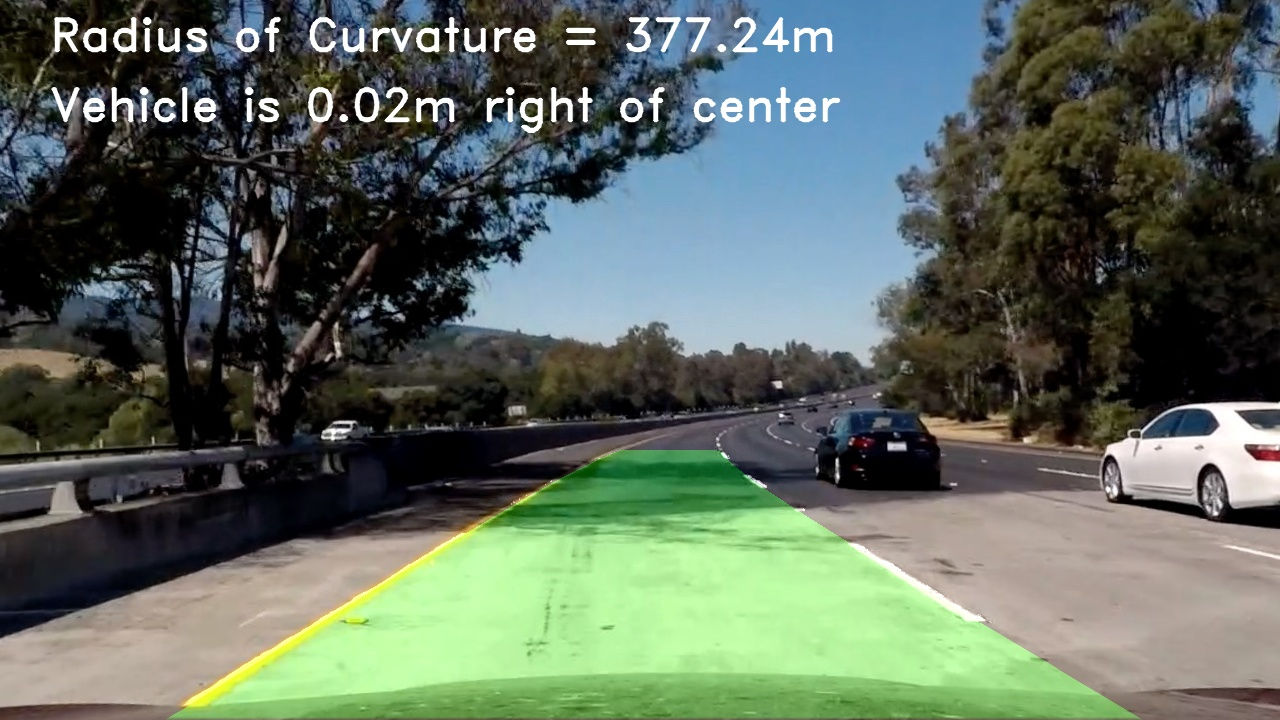
\includegraphics[width=0.75\textwidth]{../output_images/test/test5final.jpg}
\caption{Example Output Frame}
\label{fig8}
\end{center}
\end{figure}

\section{Discussion}
The part that need most calibration effort is the to create the thresholded image. When the light condition changes or more noise on the road, the resulting thresholded picture can easily include lots of unwanted frame.  To process the project video, the tree shadows create some difficulty so another restraint from the L channel in HLS space is added. But the same trick won't work on challenge video, a different set of calibration parameters in $thresholdImage$ function or update the parameters dynamically based on the overall image parameter such as lightness might work. But I could not spare more time on it. Also put all code in a overall object is another challenge for myself. I hope I have time to polish and update my code in future.

\end{document}
